\chapter{Codebase: Plotting Panel}

The plotting panel module contained in src/modules/plotDock.js is one
of the most important deliverables in the application.  It uses a
web-plotting library called 'crayon', available at 
http://g-node.github.com/crayon to create plots of the signals,
spiketrains etc, being requested.

\section{Description}

The plotting panel has a lot of data and functionality to handle.  The
primary objective is to show plots of electrophysiological data.  This
data usually comes in the following forms:

\begin{enumerate}
  \item{Signals}
  These are arrays of time and electric potential.  Usually referred
  to as analogsignals.  These objects come in two forms.  Regularly
  sampled and irregularly sampled.  The former have a well defined
  sampling rate and hence require only the time value at the start of
  the signal to be defined.  The latter on the other hand have no
  defined sampling rate and therefore require the time to be mentioned
  along with every measured electric potential value.

  \item{Spiketrains}
  These are arrays of time values specifying when the action
  potentials were fired by neurons.

  \item{Events}
  An event is an instant of time when something took place.  Eg.
  stimulation.

  \item{Epoch}
  Some events have a time duration, and therefore consist of two time
  values. Eg. Showing of a blue-screen from time a to time b.
\end{enumerate}

WDAT's plotting panel is equipped to show all data types as discussed
above. 

\begin{figure}[h!t]
  \centering
  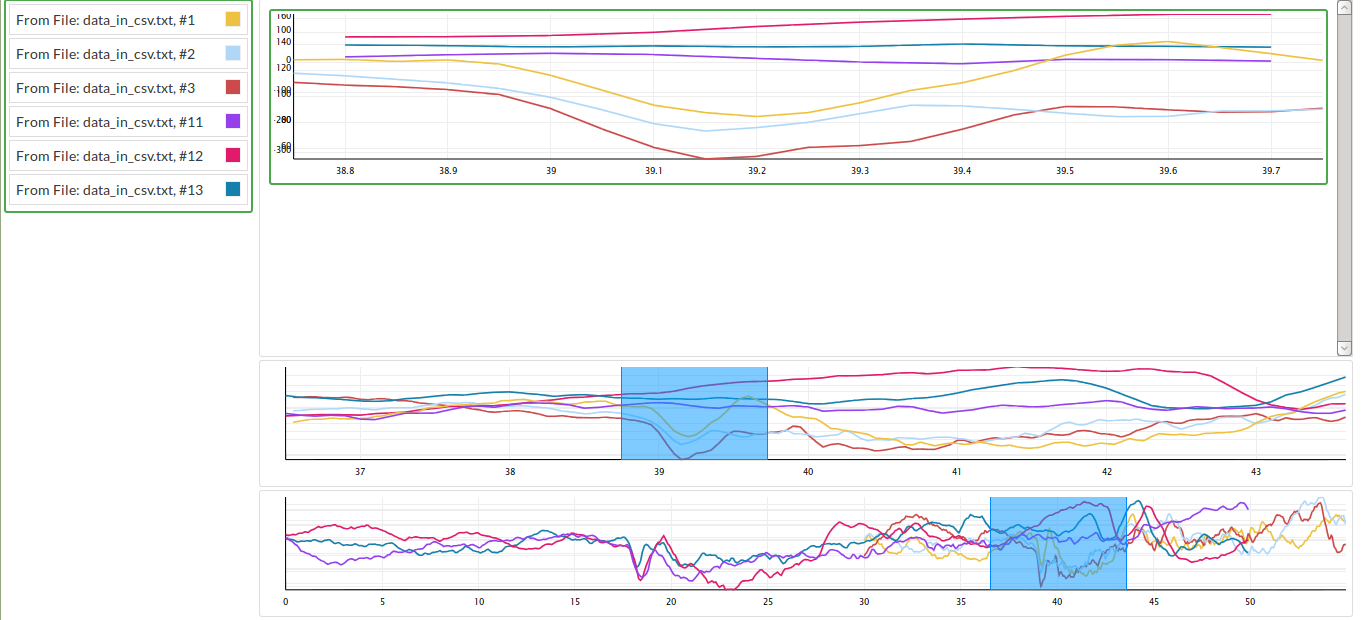
\includegraphics[width=\textwidth]{src/images/wdat-plotting-panel.png}
  \caption{Plotting Panel.}
\end{figure}

As can be seen in the figure, there are three levels of zoom in the
plotting panel.  These levels and their respective uses are defined
below.

\subsection{Total Level}

This consists of the entire time-domain of the signals' spiketrains
etc supplied.  The main use of this level is to visualize the entire
set of plottables and to identify the interesting zones.

\subsection{Zoom Level}

A small selection in the 'total' level will cause the 'zoom' level to
be activated.  The zoom level is used to narrow down the selection to
the interesting domain before isolating out the zone of maximum
relevance.

\subsection{Detail Level}

A selection in the 'zoom' level causes the 'detail' level to be
activated.  The 'detail' level is larger in height than the other two
levels and allows maximum data to be seen.  It also has a grouping
feature which allows you to group arbitrary plottables for comparison
or isolation purposes.

If the number of groups is larger than 2, the space allotted to the
detail plotting level is not enough to show all the groups.  It turns
into a scrollable area and the individual groups are contained within
this scrollable area.

\subsection{Legend}

The plots merely show the signals and spiketrains, etc.  There is no
naming of the signals within the plot since this would hamper clarity
and take up space.  The signals, spiketrain etc have unique colours
however.  This is used to denote the identity of the plottables via
the legend.  The legend module is located to the left of the plotting
panels.  It uses color-coding to denote the signals and also
color-borders to denote the groups.
